
\begin{figure*}
\centering
\begin{tabular}{cc}
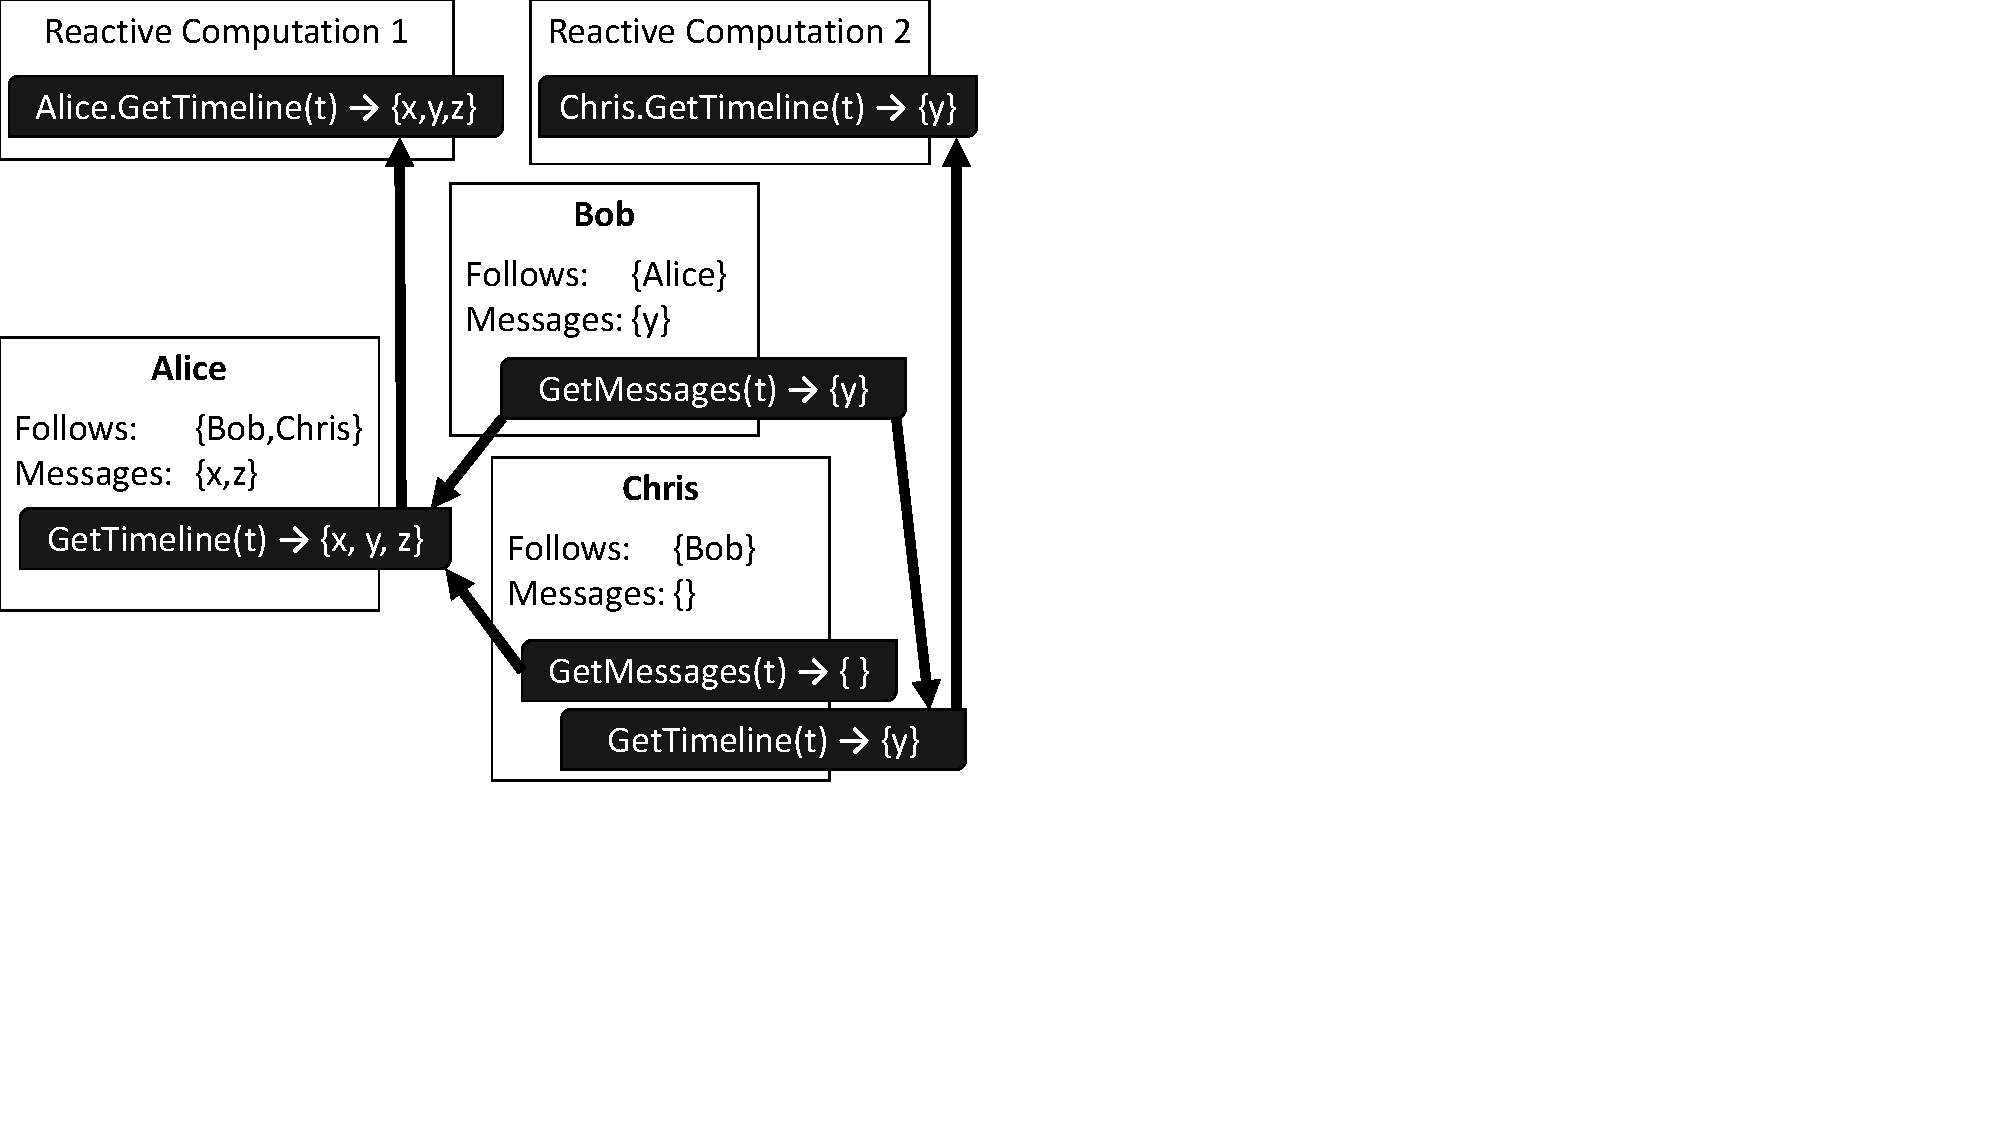
\includegraphics[scale=.45, viewport=-1 164 480 540]{figs/summaries}
&
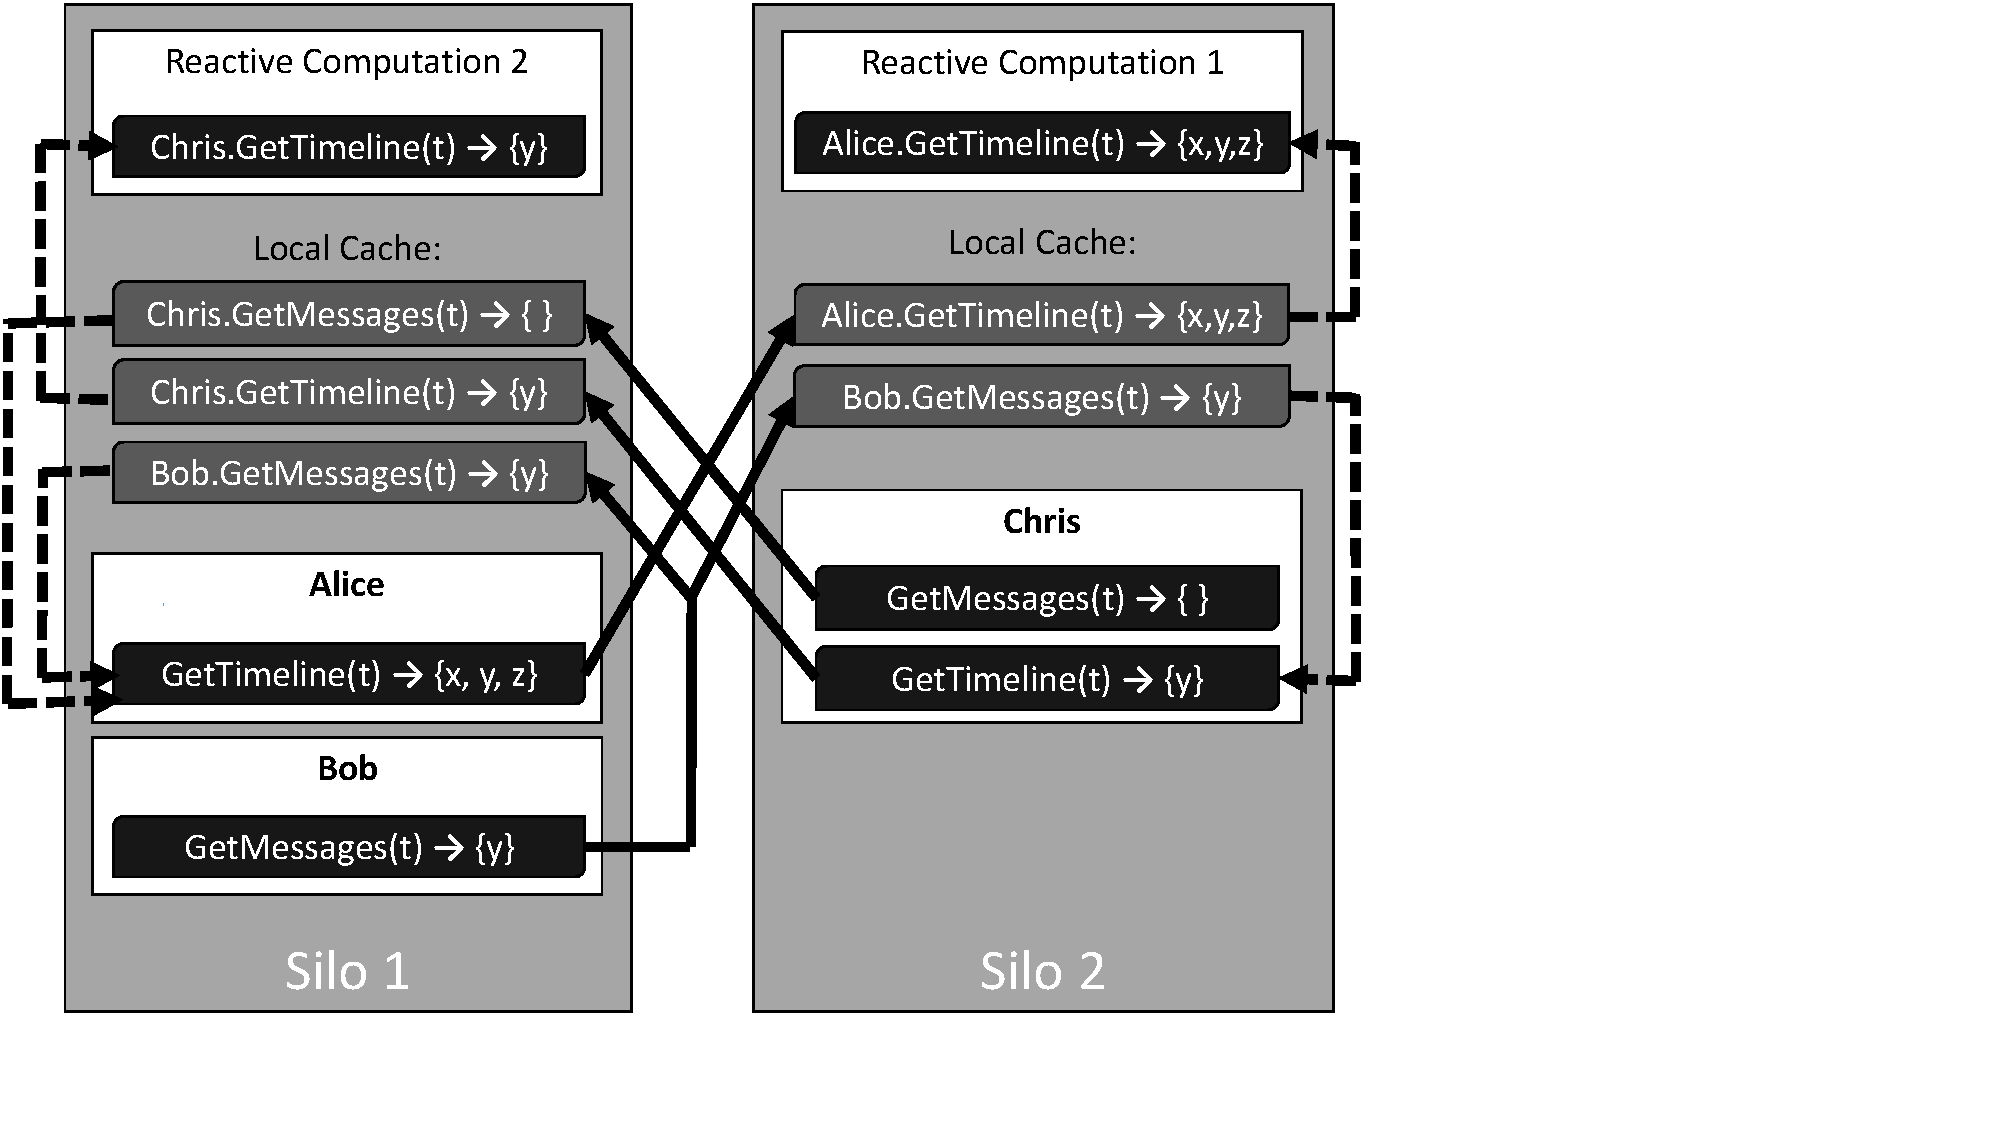
\includegraphics[scale=.4, viewport=-10 53 656 540]{figs/silos}\\
\end{tabular}
\caption{\textbf{(a)}  (on the left) example of a dependency graph of summaries, for two reactive computations; \textbf{(b)} (on the right) example of a corresponding bipartite dependency graph of summaries and local caches, distributed over two silos.}\label{fig:summaries}
\end{figure*}

\section{Algorithm}

To determine when a result of a reactive computation changes, we track all the grains it depends on. Tracking these dependencies is done entirely at runtime and does not require any static analysis: rather, we modify the virtual actor runtime to intercept grain calls and construct a \emph{dependence graph}.

We explain the nature of this dependency graph in two stages: first, we describe it as a directed ayclic graph of summaries (\S\ref{sec:summaries}). Then, we show to represent it as a bipartite graph of summaries and caches (\S\ref{sec:bp}) to improve performance and handle failures in a distributed setting. 

\subsection{Summaries and Dependencies}\label{sec:summaries}

During execution, we record and store a \emph{summary} for each executed operation. A summary is a pair consisting of (1) the invoked operation (including grain identity, method name, and all parameters), and (2) the value or exception returned at the end. For each summary, we record what other summaries it depends on, and what summaries depend on it. The result is a \emph{dependency graph} that represents the computation that was performed.

For example, consider Fig.~\ref{fig:summaries}(a). It shows a dependency graph of summaries recorded in a situation where two clients perform reactive computations \lstinline|Alice.GetTimeline(t)| and \lstinline|Chris.GetTimeline(t)| for the same time parameter \lstinline|t|. Summaries are shown as black boxes, and reside either in a grain or in a reactive computation. Summary dependencies are shown as black arrows.

\paragraph{Summary Reuse.} If a summary for a particular operation already exists, we reuse it. For example, the summary \lstinline|[GetMessages(t)->{y}]| of Bob's grain is shared: two other summaries depend on it.

\paragraph{Summary Re-execution.} If a summary is stale (see section \ref{sec:cp}), it is marked for re-execution. When re-executed, the dependencies may change, and are updated accordingly. 

\paragraph{Garbage Collection.} A summary for a grain method is deleted if there are no other summaries that depend on it.  A summary for a reactive computation is deleted when the reactive computation object is disposed. Since the dependency graph is acyclic (a cycle would represent a query with infinite recursion, which is prevented by the runtime), this means that summaries are guaranteed to be collected when no longer needed.  

\subsubsection{Change Propagation}\label{sec:cp}

We call a summary \emph{stale} if re-execution of the computation or operation would yield a different result. Our change propagation algorithm guarantees that \emph{any stale summary is eventually re-executed}, lest it disappear (i.e. fails or is removed). As we generally assume that the computations are deterministic, and because grains cannot share any state, summaries can become stale for only two reasons: either (1) the state of their grain changes, or (2) a summary they depend on becomes stale. Thus, the following is sufficient:
\begin{enumerate}
\item Whenever a grain operation changes the state of a grain, we mark all summaries of that grain for re-execution.
\item After a summary for a grain operation is re-executed, we compare the new result to the previous result. If it is the same, no further action is needed. Otherwise, we mark all dependent summaries for re-execution.
\hidden{\item After a summary for a reactive computation is re-executed, we push the new result to the consuming result tracker object.}
\end{enumerate}
 
\noindent For example, executing the operation \lstinline|Chris.Unfollow("Bob")| will mark both of the summaries in Bob's grain for re-execution. Re-execution of \lstinline|[GetMessages(t)->{}]| yields the same result, and propagation stops. But re-execution of \lstinline|[GetTimeline(t)->{y}]| yields a different result \lstinline|{}|, which means we mark the dependent summary in Reactive Computation 2, \lstinline|[Chris.GetTimeline(t)->{y}]|, for re-execution. After it re-executes, the latest result reaches the client as desired.

\paragraph{Batching. } Some time may pass in between marking a summary for re-execution and the actual re-execution. In particular, it may be marked multiple times. This batching effect can improve system throughput significantly under high update frequencies, as we demonstrate in the evaluation section.

\subsection{Silo-Local Caching}\label{sec:bp}

Under the hood, Orleans' virtual actor runtime load-balances grains across different physical machines called silos. The set of silos can change when administrators choose to increase or decrease the number of servers, or when servers fail, which is detected automatically. By design, the application layer is largely unaware of how the existence of these silos and how grains are allocated to them. However, for our algorithm, the way in which grains are distributed over silos is relevant, because (1) the latency of a remote call is orders of magnitude higher than the latency of a local call, and (2) silos can fail independently. To achieve performance and fault tolerance, we thus add an extra \emph{caching indirection layer} to the dependency graph.

Rather than having summaries that depend directly on other summaries, we let summaries depend on local caches, and those caches in turn depend on local or remote summaries. This effectively creates a bipartite dependency graph consisting of summaries and caches. We show an example in Fig.~\ref{}(b). It shows the bi-partite version of the same dependency graph as in Fig.~\ref{fig:summaries}(a). There are now two different types of edges: cache dependencies (dotted arrows), which are always within a silo, and summary dependencies (solid arrows), which may cross silo boundaries. 

\paragraph{Local Cache Hits.} When a summary is re-executed, any contained grain operations that have not changed hit in the local cache, which is implemented using a concurrent hash table. Therefore, the overhead of re-execution of summaries is tolerable: the latency of our change propagation is very close to the performance of a hand-written push-based solution, as we demonstrate in the evaluation section.

\paragraph{Back-Pressure}. 
. This is crucial for the common case where very few dependencies have changedBy keeping local caches, we make sure that the reexecution of
Change propagation along solid arrows is push-based: the new result value is sent from summaries to the corresponding caches. Change propagation along It is invalidation based along which  Change propagation along dotted arrows is based on marking

\paragraph{Failure Handling}. 

